\documentclass[a4paper,11pt]{jsarticle}


% 数式
\usepackage{amsmath,amsfonts}
\usepackage{bm}
\usepackage{physics}
% 画像
\usepackage[dvipdfmx]{graphicx}
% ローマ数字
\usepackage{otf}
% 単位
\usepackage{siunitx}
% 表
\usepackage{multirow}
% 化学反応
\usepackage[version=4]{mhchem}


\begin{document}

\title{理論演習 べき減衰の考察,定常解との比較,濃度依存エラー率の導入}
\author{齋藤駿一}
\date{\today 編集}
\maketitle

ここでは,反応を$[\text{反応物}, \text{生成物}, \text{触媒}]$という形で表し,これをまとめた形で反応ネットを表記する.

\section{反応ネットと時系列の確認}
ゴミと複合体の間の反応速度は,$\epsilon_p = 1, \epsilon_m=0.01$とした.
まず,時刻$t=10^5$における栄養濃度と成長速度の関係をプロットした.
その結果,エラー率0,0.01,0.1,1でそれぞれ図\ref{fig:err0_ng_reac},図\ref{fig:err001_ng_reac},図\ref{fig:err01_ng_reac},図\ref{fig:err1_ng_reac}が得られた.
また,エラー率0において,低栄養濃度での成長に失敗しているある反応ネット($[[1,0,0], [0,1,0]]$)の時間発展は図\ref{fig:err0_tc_reac1}のようになった.

このべき減衰は,この反応ネットに対応する微分方程式に$x_0=Ct^\alpha$を代入することで導ける.
具体的には,一次近似として$x_1 = 1$と見なすと$\alpha = -1$がいえ,これをもとにすると
\begin{align}
  x_0 &= \frac{C}{t} \\
  x_1 &= 1 - \frac{1-2C}{t}
\end{align}
が導ける.
後者の式を確認するため,$1-x_1$をプロットすると,予想通り$t^{-1}$で減衰する結果が得られた(図\ref{fig:err0_tc_reac1_check}).

逐一確認することはできなかったが,エラー率1,時刻$t=10^5$のときの図\ref{fig:err1_ng_reac}を$t=10^6$まで時間発展させると図\ref{fig:err1_ng_reac_check_T6}となったことから,他の図も同様の理由で減衰しきっていないだけと考えられる.

一方で,エラー率0において,反応ネット$[[1,0,0]]$に対応する微分方程式の定常状態を解析的に解くと,今回のパラメータでは
\begin{equation}
  x_0 = \frac{\sqrt{1+8n} - 3}{4}
\end{equation}
が得られた.
これとシミュレーションの結果を比較すると,よく合っていることが確認できた(図\ref{fig:err0_ng_reac_1_2_s}).
よって,図\ref{fig:err0_ng_reac}は減衰しきった結果であると考えられる.

\begin{figure}[htbp]
  \centering
  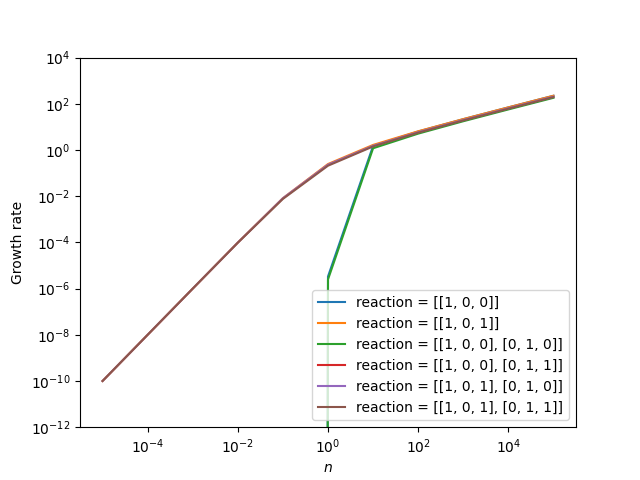
\includegraphics[width=10cm]{waste_err0_ng_reac.png}
  \caption{エラー率0のときの,$t=10^5$での栄養濃度と成長速度の関係.}
  \label{fig:err0_ng_reac}
\end{figure}

\begin{figure}[htbp]
  \centering
  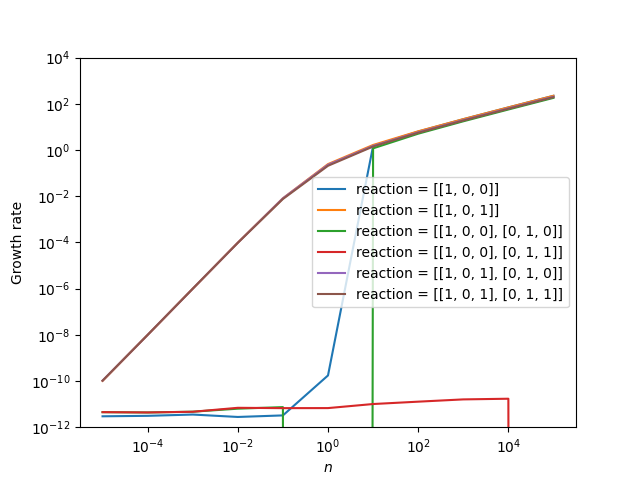
\includegraphics[width=10cm]{waste_err001_ng_reac.png}
  \caption{エラー率0.01のときの,$t=10^5$での栄養濃度と成長速度の関係.}
  \label{fig:err001_ng_reac}
\end{figure}

\begin{figure}[htbp]
  \centering
  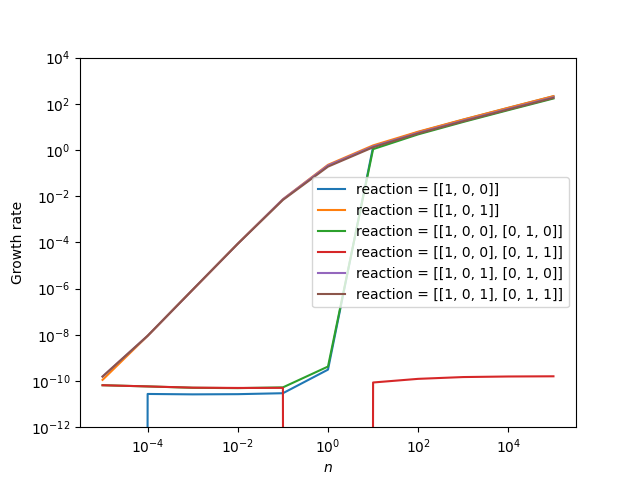
\includegraphics[width=10cm]{waste_err01_ng_reac.png}
  \caption{エラー率0.1のときの,$t=10^5$での栄養濃度と成長速度の関係.}
  \label{fig:err01_ng_reac}
\end{figure}

\begin{figure}[htbp]
  \centering
  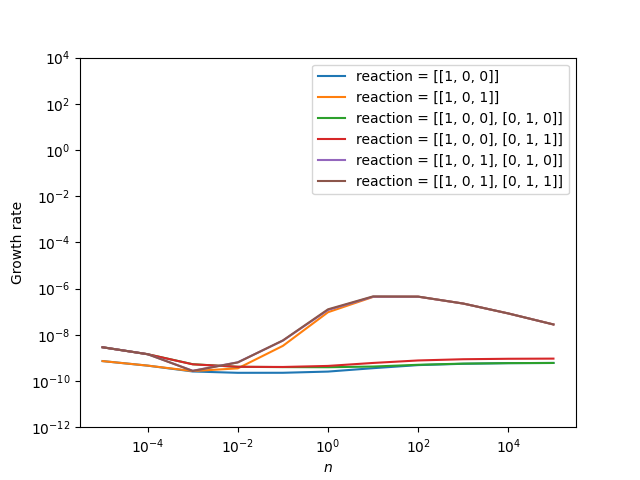
\includegraphics[width=10cm]{waste_err1_ng_reac.png}
  \caption{エラー率1のときの,$t=10^5$での栄養濃度と成長速度の関係.}
  \label{fig:err1_ng_reac}
\end{figure}

\begin{figure}[htbp]
  \centering
  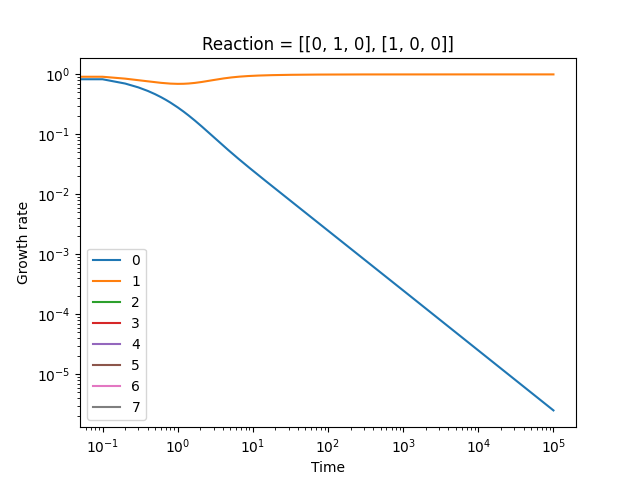
\includegraphics[width=10cm]{waste_err0_tc_reac1.png}
  \caption{エラー率0のときの,反応ネット$[[1,0,0],[0,1,0]]$の時間発展.べき減衰が見られる.}
  \label{fig:err0_tc_reac1}
\end{figure}

\begin{figure}[htbp]
  \centering
  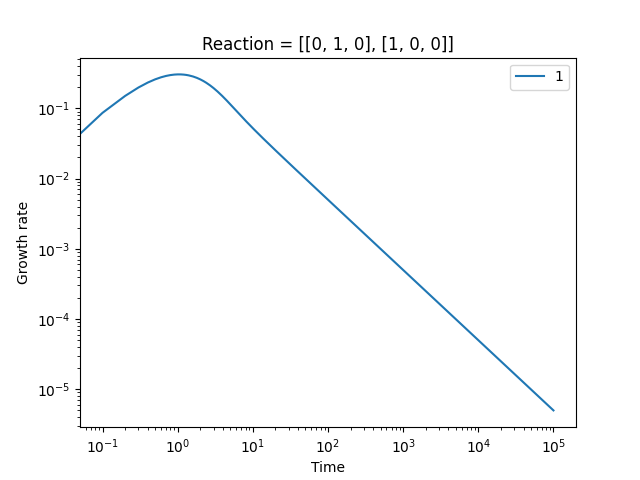
\includegraphics[width=10cm]{waste_err0_tc_reac1_check.png}
  \caption{エラー率0のときの,反応ネット$[[1,0,0],[0,1,0]]$での,$1-x_1$の時間発展.たしかに$t^{-1}$で減っている.}
  \label{fig:err0_tc_reac1_check}
\end{figure}

\begin{figure}[htbp]
  \centering
  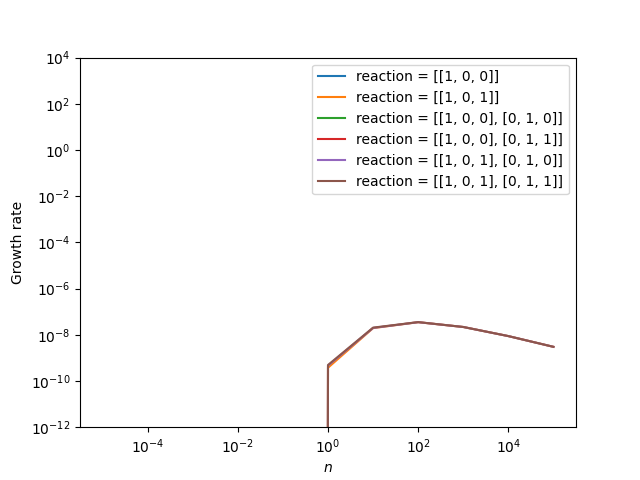
\includegraphics[width=10cm]{waste_err1_ng_reac_check_T6.png}
  \caption{エラー率1のときの,$t=10^6$での栄養濃度と成長速度の関係.}
  \label{fig:err1_ng_reac_check_T6}
\end{figure}

\begin{figure}[htbp]
  \centering
  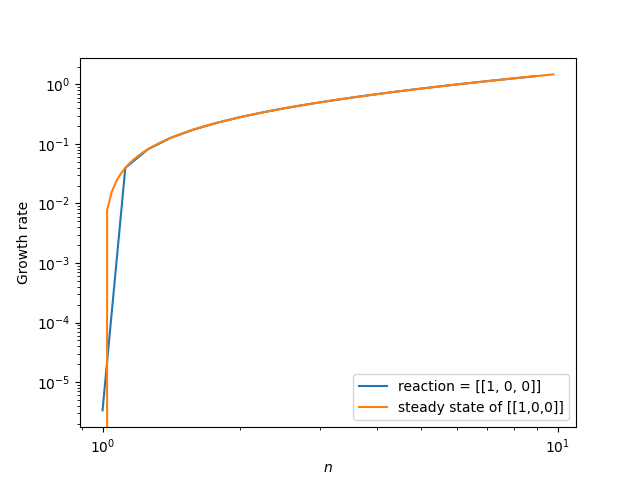
\includegraphics[width=10cm]{waste_err0_ng_reac1_2_s.png}
  \caption{エラー率0におけるシミュレーション結果と,解析的に導いた定常状態との比較.}
  \label{fig:err0_ng_reac_1_2_s}
\end{figure}

\newpage

\section{エラー率を内部代謝物の濃度に依存させたモデル}

以上の結果を踏まえて,エラー率を膜分子濃度$x_0$または栄養分子濃度$x_1$に依存させたモデルを考えた.
具体的には,エラー率$e$を
\begin{equation}
  e = \frac{\delta}{1+x} \qquad x = x_0 \,\mathrm{or}\, x_1 
\end{equation}
とした.
(ただし,$0<\delta<1$とする.)

シミュレーションの結果,適当に選んだ値では,エラー率がどちらの分子に依存するか($x=x_0$か$x=x_1$か)によらずほとんど同じ挙動が見られた(図\ref{fig:errslp01_tc_reac1_n10},図\ref{fig:errslp01_tc_reac1_n1}).

\begin{figure}[htbp]
  \centering
  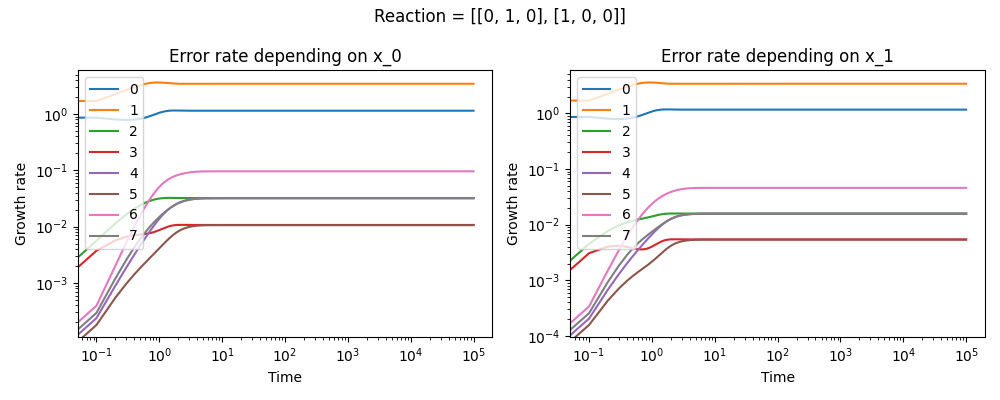
\includegraphics[width=\columnwidth]{waste_errslp01_tc_reac1_n10.png}
  \caption{$\delta=0.1$,栄養濃度$n=10$における,反応ネット$[[1,0,0],[0,1,0]]$の各成分の時間発展.エラー率が膜分子に依存するときも栄養分子に依存するときも生存するという例.}
  \label{fig:errslp01_tc_reac1_n10}
\end{figure}

\begin{figure}[htbp]
  \centering
  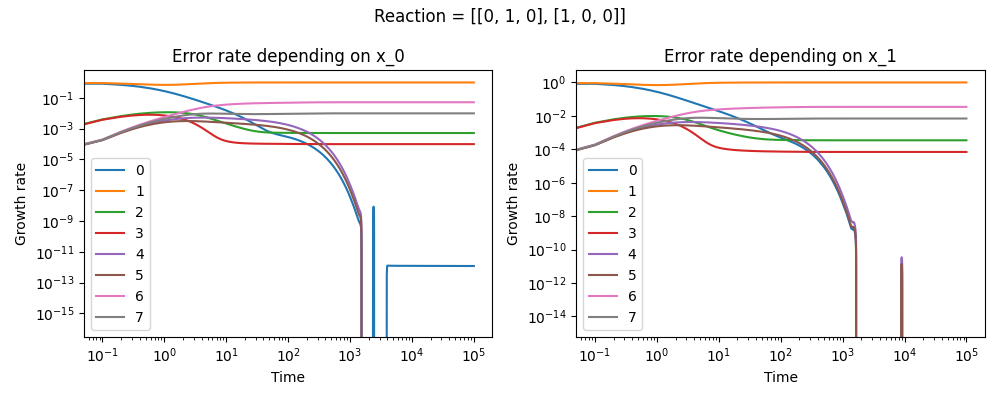
\includegraphics[width=\columnwidth]{waste_errslp01_tc_reac1_n1.png}
  \caption{$\delta=0.1$,栄養濃度$n=1$における,反応ネット$[[1,0,0],[0,1,0]]$の各成分の時間発展.エラー率が膜分子に依存するときも栄養分子に依存するときも生存しないという例.}
  \label{fig:errslp01_tc_reac1_n1}
\end{figure}

しかし,ある反応ネットでは,パラメータをうまく調整すると,$x=x_0$と$x=x_1$で異なる挙動を示した.
とくに,反応ネットとして$[[1,0,0],[0,1,0]]$または$[[1,0,0]]$を考えたとき,経験的に,「栄養濃度を$n=1+\delta$とおくと,$x=x_0$のとき生存せず(どこかで$x_0=0$となり),$x=x_1$のとき生存する($x_0$が有限値に収束する)」という法則が確認できた.
ただしこの法則は,反応ネット$[[1,0,1]]$では確認できなかった.
おそらく,この法則が成立する反応ネットは,図\ref{fig:err0_ng_reac}において$n=1$で成長率が急降下している2つに限られると考えられる.

\begin{figure}[htbp]
  \centering
  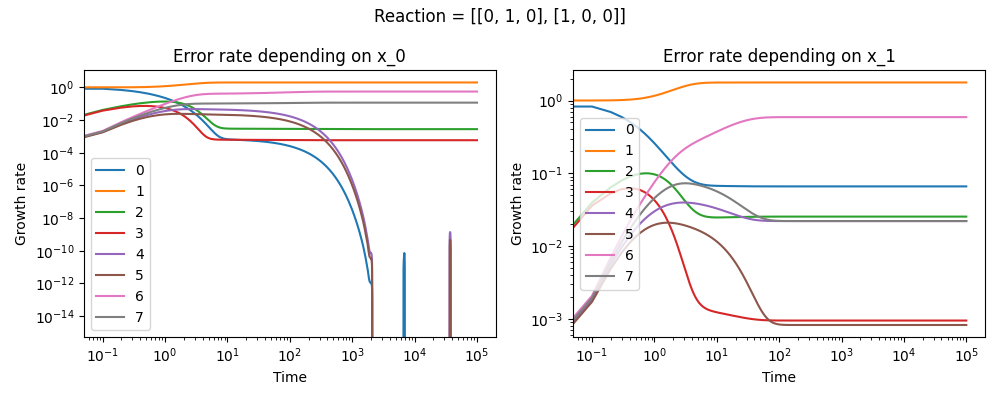
\includegraphics[width=\columnwidth]{waste_errslp1_tc_reac1_n2.png}
  \caption{$\delta=1$,栄養濃度$n=2$における,反応ネット$[[1,0,0],[0,1,0]]$の各成分の時間発展.エラー率が膜分子に依存するときは生存しないが,栄養分子に依存するときは生存するという例.}
  \label{fig:errslp1_tc_reac1_n2}
\end{figure}

\begin{figure}[htbp]
  \centering
  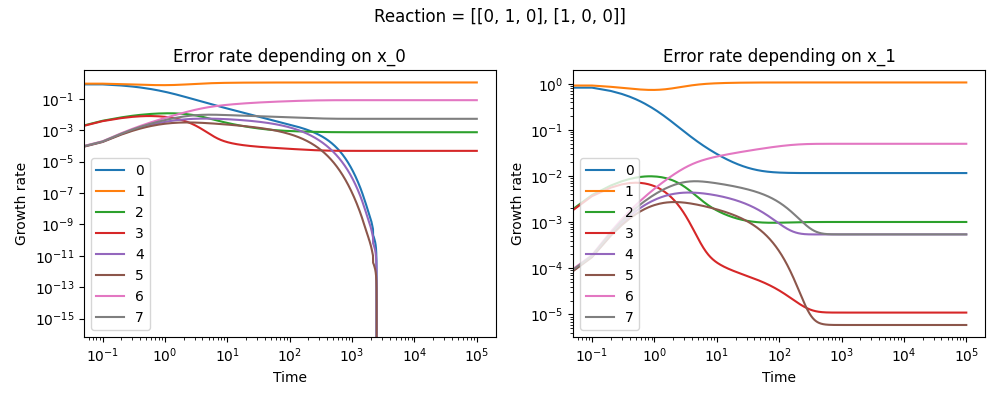
\includegraphics[width=\columnwidth]{waste_errslp01_tc_reac1_n11.png}
  \caption{$\delta=0.1$,栄養濃度$n=1.1$における,反応ネット$[[1,0,0],[0,1,0]]$の各成分の時間発展.エラー率が膜分子に依存するときは生存しないが,栄養分子に依存するときは生存するという例.}
  \label{fig:errslp01_tc_reac1_n11}
\end{figure}

\begin{figure}[htbp]
  \centering
  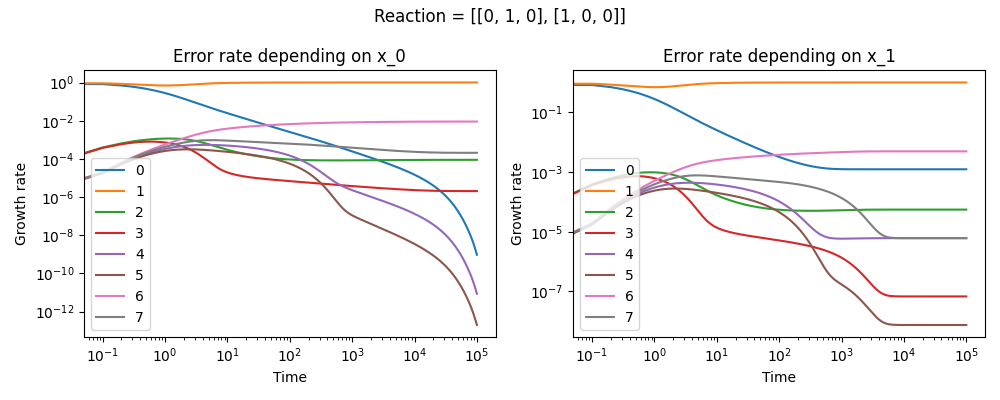
\includegraphics[width=\columnwidth]{waste_errslp001_tc_reac1_n101.png}
  \caption{$\delta=0.01$,栄養濃度$n=1.01$における,反応ネット$[[1,0,0],[0,1,0]]$の各成分の時間発展.エラー率が膜分子に依存するときは生存しないが,栄養分子に依存するときは生存するという例.}
  \label{fig:errslp001_tc_reac1_n101}
\end{figure}

\end{document}